\section{LMS}
LMS is a form of adaptive filter.
It works by reducing the average power of the feedback signal by modifying the coefficients in a Finite Impulse Response (FIR) filter.
An example implementation is shown below in figure~\ref{fig:lmsfilter}.
In this implementation the LMS algorithm will be used as the block labelled ``Adaptation algorithm''.
This version also aims for a slightly different effect to the method that will be employed in this project.
This project will be feeding the inverse of the noise estimate, -\^{n}(m), to the listener in order to generate the cancelling in their ear, rather than to remove the noise inside the software.

\begin{figure}[H]
	\centering
	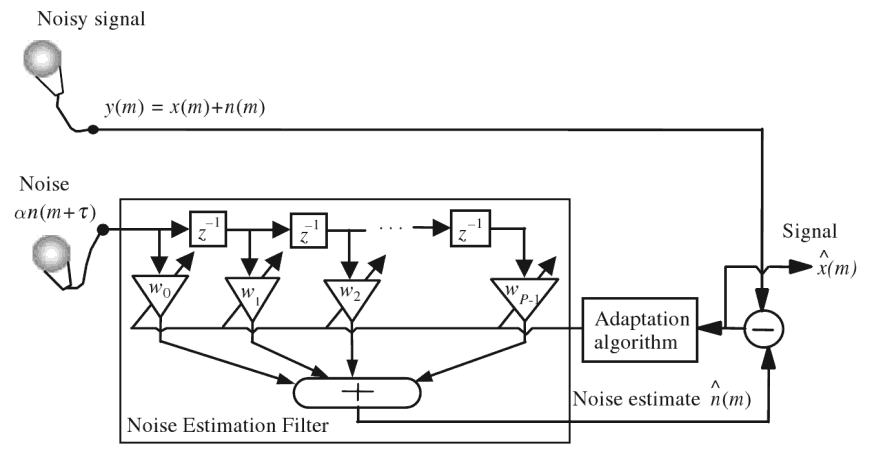
\includegraphics[width=\textwidth]{./img/lmsfilter.png}
	\caption{An example setup for the use of an LMS filter in noise cancellation (Sourced from Advanced Digital Signal Processing and Noise Reduction \cite{AdvancedDSPing})}
	\label{fig:lmsfilter}
\end{figure}


